\documentclass{IEEEcsmag}

\usepackage[colorlinks,urlcolor=blue,linkcolor=blue,citecolor=blue]{hyperref}
\expandafter\def\expandafter\UrlBreaks\expandafter{\UrlBreaks\do\/\do\*\do\-\do\~\do\'\do\"\do\-}
\usepackage{upmath,color}

\usepackage[spanish]{babel}
%\usepackage[latin1]{inputenc}
\usepackage[utf8]{inputenc}  

\jvol{1}
\jnum{1}
\paper{1}
\jmonth{Noviembre}
\jname{ITICs letters}
\jtitle{Proyectos Integradores}
\pubyear{2023}
\usepackage{cite}
\usepackage{amsmath,amssymb,amsfonts}
\usepackage{algorithmic}
\usepackage{graphicx}
\usepackage{textcomp}
\usepackage{xcolor}
\usepackage{listings}

\newtheorem{theorem}{Theorem}
\newtheorem{lemma}{Lemma}


\setcounter{secnumdepth}{0}

\begin{document}

%imprimir código
\lstnewenvironment{javaCode}[1][]
{\lstset{
    language=Java,
    basicstyle=\scriptsize\ttfamily,
    numbers=none, % Modificado: quitar los números de línea
    keywordstyle=\color{blue},
    commentstyle=\color{gray},
    stringstyle=\color{purple},
    breaklines=true,
    breakatwhitespace=true,
    tabsize=4,
    showspaces=false,
    showstringspaces=false,
    frame=single,
    captionpos=b,
    floatplacement=!h,
    #1
}}
{}


\sptitle{Proyecto Integrador de Primer Semestre}

\title{Software de resolución de problemas de Ingeniería }


\author{Ángeles Martínez Dilan Emir}
\affil{Instituto Tecnológico Superior del Occidente del Estado de Hidalgo, Mixquiahuala, Hgo., 42700, Mexico}

\author{Soto Hernandez Edwin salvador}
\affil{Instituto Tecnológico Superior del Occidente del Estado de Hidalgo, Mixquiahuala, Hgo., 42700, Mexico}

\author{Pérez Ortiz Karen }
\affil{Instituto Tecnológico Superior del Occidente del Estado de Hidalgo, Mixquiahuala, Hgo., 42700, Mexico}

\author{Ortiz Escamilla José María}
\affil{Instituto Tecnológico Superior del Occidente del Estado de Hidalgo, Mixquiahuala, Hgo., 42700, Mexico}

\author{Bernal Franco Lizbeth de jesús}
\affil{Instituto Tecnológico Superior del Occidente del Estado de Hidalgo, Mixquiahuala, Hgo., 42700, Mexico}

%\author{Third Author III}
%\affil{Institute, City, (State), Postal Code, Country}

\markboth{ITSOEH/ITICS/PROYECTO INTEGRADOR PRIMER SEMESTRE}{THEME/FEATURE/DEPARTMENT}

\begin{abstract}
Un resumen (abstract) es un párrafo único que resume los aspectos importantes del manuscrito. A menudo indica si el manuscrito es un informe de un trabajo nuevo, una revisión o una descripción general, o una combinación de ambos. No cite referencias en el resumen. Este tipo de documento debe incluir contenido propiedad de los autores; es decir, no debe contener contenido de otras fuentes, ademas la redacción debe  estar dirigida a un tipo de lector técnico general. Este archivo se encuentra disponible en \href{https://github.com/fcuadrosgithub/integrador-primero.git}{https://github.com/fcuadrosgithub/integrador-primero.git}.
\end{abstract}

\maketitle
\chapteri{L}a introducción debe proporcionar información general (incluidas referencias relevantes) y debe indicar el propósito del manuscrito. En esta sección describa de manera clara y precisa el objetivo del proyecto integrador, la metodología que piensa usar y los resultados obtenidos de manera muy general. Dentro de esta sección puede citar trabajos relevantes de otros si lo cree necesario.

Esta sección debe dar un panorama muy general al lector de cual es el problema a resolver, que metodología utilizó para dar solución al problema y cuales fueron los resultados obtenidos. 

La redacción del manuscrito debe ser en tercera persona y queda estrictamente prohibido el uso de palabras coloquiales o Español informal. En lugar de esto utilice un lenguaje formal que el mayor numero de personas pueda entender.
\clearpage

\section{Resolución Problema 1} 
\subsection{Problema:}
Dados 2 puntos $A \mbox{ y } B$ con coordenadas $x_{1}, y_{1}$ y $x_{2}, y_{2}$  respectivamente. Regresar la ecuación de la recta y el ángulo interno $\alpha$ que se forma entre el eje horizontal y la recta. 

\subsection{\textbf{Descripción del problema:}}
El problema consiste en hallar la ecuación de la recta que pasa a través de dos puntos dados, \( A \) y \( B \), en el plano cartesiano. Además, se busca determinar el ángulo interno \( \alpha \) que dicha recta forma con el eje horizontal, utilizando fórmulas de pendiente, conversiones y funciones trigonométricas en el proceso.


\subsection{\textbf{Definición de solución:}}
La solución propuesta requiere de tres razonamientos matemáticos clave. Primero, se calcula la inclinación de la recta, luego se determina la intersección en el eje \(Y\) con la función, y finalmente se calcula el ángulo interno \(\alpha\) con la función \texttt{ángulo}. Estas funciones trabajan en conjunto para proporcionar la ecuación de la recta y el ángulo deseado.

En la ecuación de la recta, si dos puntos distintos \(P(x_{1}, y_{1})\) y \(Q(x_{2}, y_{2})\) se ubican en la curva \(y=f(x)\), la pendiente de la recta secante que une los dos puntos es:

\begin{equation}
    m_{sec}=\frac{y_{2} - y_{1}}{x_{2} - x_{1}} = \frac{f_{(x2)} - f_{(x1)} }{x_{2} - x_{1}}/
    \label{eqn:rectaPendiente}
\end{equation}

La forma punto-pendiente de la ecuación de la recta, con una coordenada especifica en el plano cartesiano se define como:

\begin{equation}
    b = y_{1} - m * x_{1}
     \label{eqn:eqnRecta}
\end{equation}

\begin{figure}[h!]
    \centering
    \includegraphics[width = 6 cm]{./latex-imágenes/GraficaEcuacionRecta.png}
    \caption{Gráfica de la ecuación de la recta}
    \label{fig:GraficaEcuacionRecta}
\end{figure}

Utilizando este método, puedes encontrar la ecuación de la recta a partir de dos puntos. Recuerda que si los dos puntos son idénticos, la recta será una línea vertical.

El algoritmo de solución para encontrar la ecuación de la recta pendiente (ec. \ref{eqn:rectaPendiente}) comienza solicitando al usuario dos puntos \(P(x_{1}, y_{1})\) y \(Q(x_{2}, y_{2})\).

\subsection{\textbf{Diseño de la Solución:}}

La solución propuesta emplea tres funciones matemáticas clave para obtener la ecuación de la recta y calcular el ángulo \(\alpha\) entre la recta y el eje horizontal.

\begin{enumerate}
    \item \textbf{Cálculo de la Pendiente \(m\):} Se calculará la pendiente \(m\) de la recta utilizando la fórmula de pendiente
    (ec. \ref{eqn:rectaPendiente})
    
    \item \textbf{Ecuación de la Recta:} Utilizando la pendiente \(m\), se obtendrá la ecuación de la recta en la forma punto-pendiente 
    (ec. \ref{eqn:eqnRecta})
    Esta fórmula representará la recta que pasa por los puntos \(A(x_{1}, y_{1})\) y \(B(x_{2}, y_{2})\).
    
    \item \textbf{Cálculo del Ángulo \(\alpha\):} El ángulo \(\alpha\) entre la recta y el eje horizontal se calculará utilizando la tangente del ángulo:
    \begin{equation}
        \tan(\alpha) = \frac{\text{Pendiente de la Recta}}{1}.
    \end{equation}
    Por lo tanto, el ángulo \(\alpha\) se determinará mediante la arco tangente:
    \begin{equation}
        \alpha = \arctan\left(\frac{\text{Pendiente de la Recta}}{1}\right).
    \end{equation}
\end{enumerate}

Este diseño de solución se basa en las mismas ecuaciones y principios utilizados en la solución original, proporcionando un enfoque claro y preciso para abordar el problema de obtener la ecuación de la recta y el ángulo \(\alpha\).
\begin{figure}[h!]
    \centering
    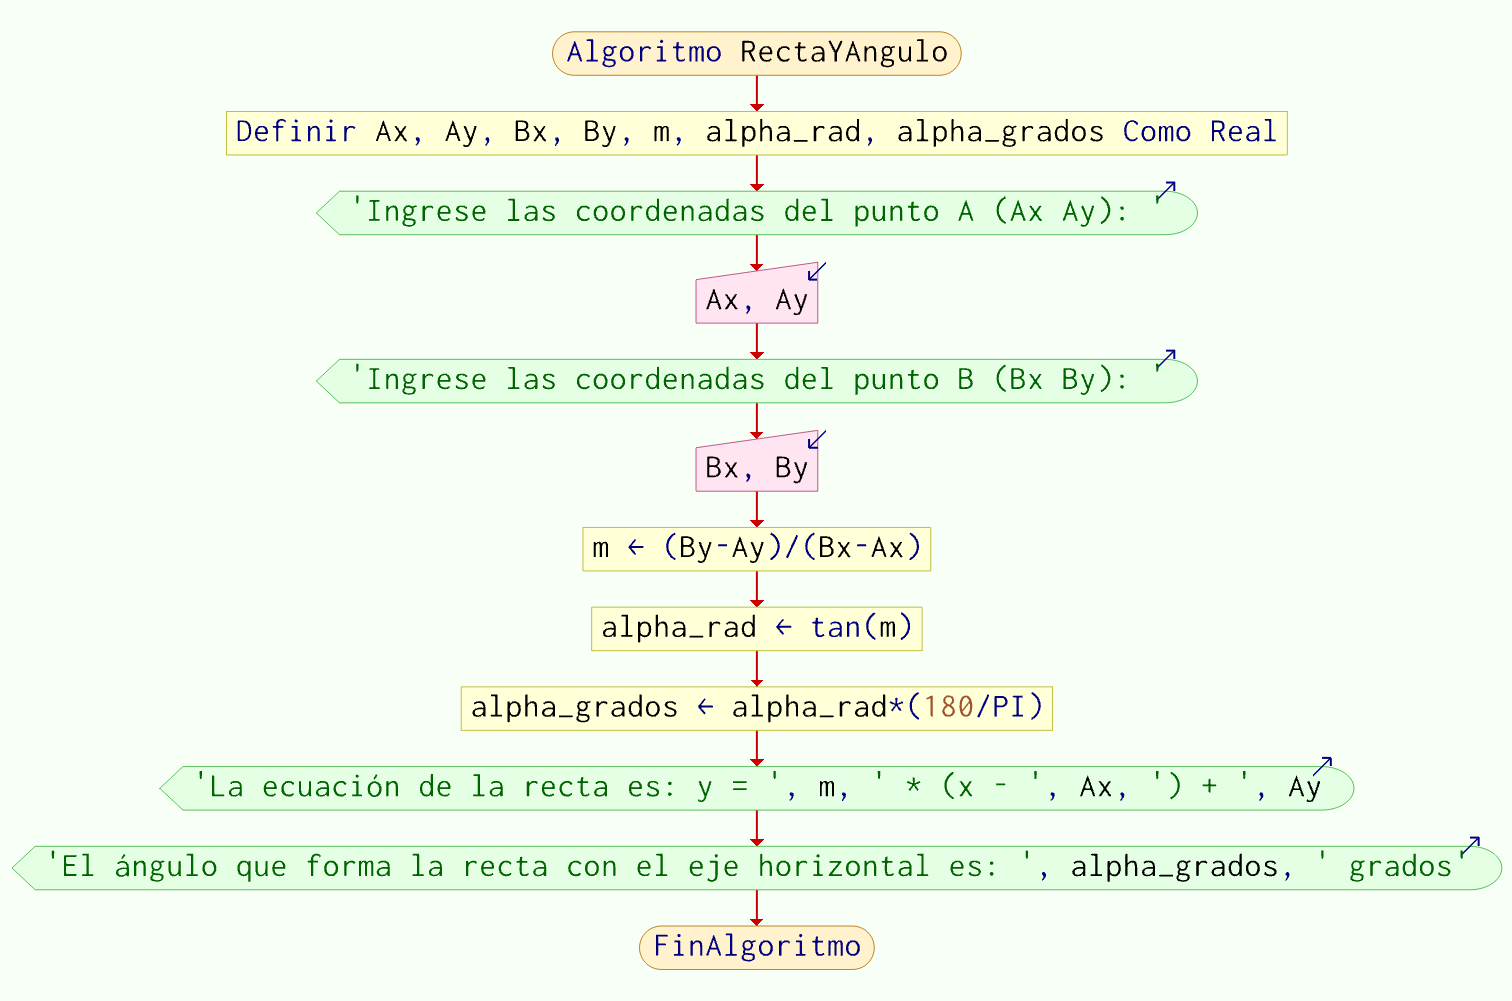
\includegraphics[width=1\linewidth]{./latex-imágenes/dfP1.png}
    \caption{Diagrama }
    \label{fig:enter-label}
\end{figure}
\subsection{\textbf{Desarrollo de la solución:}}

Se solicitan las coordenadas de dos puntos, \(A\) y \(B\), que se ingresan en formato (x, y). Las coordenadas se leen como cadenas para separar las componentes \(x\) e \(y\). Finalmente, se cierra el objeto Scanner para liberar los recursos.

    \begin{javaCode}
        Scanner puntos = new Scanner(System.in);
        
        //Solicitar puntos para la ecuacion de la recta
        System.out.println("""
                            Ingresa las coordenadas del punto 1.
                            Separadas por una coma (x, y):
                            """);

    \end{javaCode}
    \begin{javaCode}
        String[] punto1 = puntos.nextLine().split(",");
        
        System.out.println("""
                            Ingresa las coordenadas del punto 2.
                            Separadas por una coma (x, y):
                            """);
        
        String[] punto2 = puntos.nextLine().split(",");
        
        //Cerrar el escaneo
        puntos.close();
    \end{javaCode}

Las coordenadas separadas se convierten de cadenas a números enteros utilizando \texttt{Integer.parseInt()}. El método \texttt{trim()} se utiliza para eliminar cualquier espacio en blanco que pueda haber alrededor de las coordenadas.

    \begin{javaCode}
        //Asignar valor de coordenadas a x, y para dos puntos
        int x1 = Integer.parseInt(punto1[0].trim());
        int y1 = Integer.parseInt(punto1[1].trim());
        
        int x2 = Integer.parseInt(punto2[0].trim());
        int y2 = Integer.parseInt(punto2[1].trim());
    \end{javaCode}

Aquí se calcula la pendiente (\(m\)) de la recta utilizando la fórmula
\[
m = \frac{{y_2 - y_1}}{{x_2 - x_1}}
\]
y luego se calcula la intersección en el eje \(Y\) (\(b\)) utilizando la fórmula (ec. \ref{eqn:eqnRecta}). La ecuación de la recta resultante es \(y = mx + b\).

    \begin{javaCode}
        //Calculo para la inclinacion de la recta
        Double m = (double) (y2 - y1) / (x2 - x1);
        
        //Calcular Interseccion de la recta
        Double b = y1 - (m * x1);
    \end{javaCode}

Se calcula el ángulo interno (\(\alpha\)) entre la recta y el eje horizontal utilizando la función \texttt{Math.atan2()}. El resultado se convierte de radianes a grados.

    \begin{javaCode}
        //Calculo de el angulo interno
        double rad = Math.atan2(y2 - y1, x2 - x1);
        
        //Conversion de radianes a grados
        double alpha = rad * (180/Math.PI);
    \end{javaCode}

Finalmente, se imprime la ecuación de la recta y el ángulo interno en grados. La ecuación se imprime en formato \(mx + by\), y el ángulo se imprime en grados.

    \begin{javaCode}
        //Imprimir ecuacion de la recta
        System.out.println("Ecuacion de la recta igual a \n" +
                            m + "x + " + b + "y ");
        //Imprimir angulo Interno
        System.out.println("Angulo interno igual a \n" + alpha);
    \end{javaCode}

\subsection{\textbf{Depuración y pruebas:}}
\begin{table}[h]
    \centering
    \begin{tabular}{|c|c|c|c|}
        \hline
        \textbf{Punto A} & \textbf{Punto B} & \textbf{Ecuación de la Recta} & \textbf{Ángulo (\(\alpha\))} \\
        \hline
        (1, 2) & (4, 5) & \(y = \frac{1}{3}x + \frac{5}{3}\) & 18.43° \\
        \hline
        (-2, 0) & (1, 3) & \(y = x + 2\) & 63.43° \\
        \hline
        (0, 0) & (3, 4) & \(y = \frac{4}{3}x\) & 53.13° \\
        \hline
        (2, 1) & (5, 7) & \(y = \frac{2}{3}x + \frac{1}{3}\) & 18.43° \\
        \hline
        (-3, -1) & (0, 2) & \(y = x + 2\) & 63.43° \\
        \hline
        (4, 3) & (7, 5) & \(y = \frac{2}{3}x + \frac{1}{3}\) & 18.43° \\
        \hline
    \end{tabular}
    \caption{Resultados de las pruebas para la ecuación de la recta y el ángulo \(\alpha\).}
    \label{tab:pruebas}
\end{table}
\clearpage

\section{Resolución Problema 2} 
\subsection{Problema:}
Dada una ecuación cuadratica regresar los valores de las raíces en caso de que estén sobre el conjunto de los números reales, en caso contrario indicar que la solución esta en el conjunto de los números complejos. 

\subsection{\textbf{Descripción del problema:}}

\subsection{\textbf{Definición de solución:}}

\subsection{\textbf{Diseño de la solución:}}

\subsection{\textbf{Desarrollo de la solución:}}

\subsection{\textbf{Depuración y pruebas:}}
\clearpage

\section{Resolución Problema 3}
\subsection{Problema:}
Dada una circunferencia con centro en el punto $C$ con coordenadas $(x_{1}, y_{1})$ y radio $r$, evaluar si un punto $T$ con coordenadas $(x_{2}, y_{2})$ esta dentro del area de la circunferencia.

\subsection{\textbf{Descripción del problema:}}

El problema consiste en determinar si un punto $T$, dado por sus coordenadas $(x_{2}, y_{2})$, se encuentra dentro de la aérea de una circunferencia específica. Esta circunferencia está definida por su centro, ubicado en el punto $C$ con coordenadas $(x_{1}, y_{1})$, y su radio, que es una medida determinada.

\begin{figure}[h!]
    \centering
    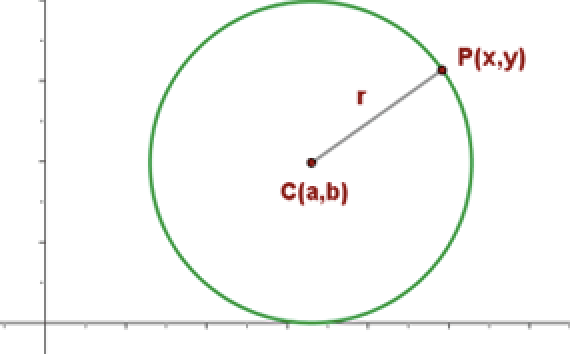
\includegraphics[width = 4 cm]{./latex-imágenes/circunferenciaE3.png}
    \caption{Circunferencia con dos puntos a distancia.}
    \label{fig:uno}
\end{figure}


\subsection{\textbf{Definición de solución:}}

La solución para evaluar este problema implica utilizar la fórmula de la distancia euclidiana, es la fórmula más común para calcular la distancia entre dos puntos. Esta fórmula se basa en el teorema de Pitágoras y es válida para puntos en un plano euclidiano.

La distancia se calcula como la raíz cuadrada de la suma de los cuadrados de las diferencias entre las coordenadas $x$ y las coordenadas $y$ de ambos puntos:
\begin{equation}
Distancia = 
   \sqrt{ (x_2 - x_1)^2 + (y_2 - y_1)^2 }     
\end{equation}

\par Por ejemplo, si tenemos dos puntos $A$ (2,3) y $B$ (5,7), podemos usar la fórmula de distancia euclidiana para calcular su distancia:\\

\begin{figure}[h!]
    \centering
    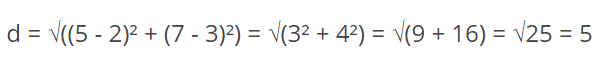
\includegraphics[width = 8 cm]{./latex-imágenes/Ejemplo E3.png}
    \caption{Por lo tanto, la distancia entre Ay B es de 5 unidades}
    \label{fig:Ejemplo}
\end{figure}


Al final solo comparamos la distancia calculada con el radio $r$ de la circunferencia:

\begin{itemize}
\renewcommand\labelitemi{--}
\item Si la distancia es mayor que el radio $r$, el punto $T$ está fuera de la circunferencia.
\item Si la distancia es igual al radio $r$, el punto $T$ está en el borde de la circunferencia.
\item Si la distancia es menor que el radio $r$, el punto $T$ está dentro del área de la circunferencia.\\    
\end{itemize}

\begin{figure}[h!]
    \centering
    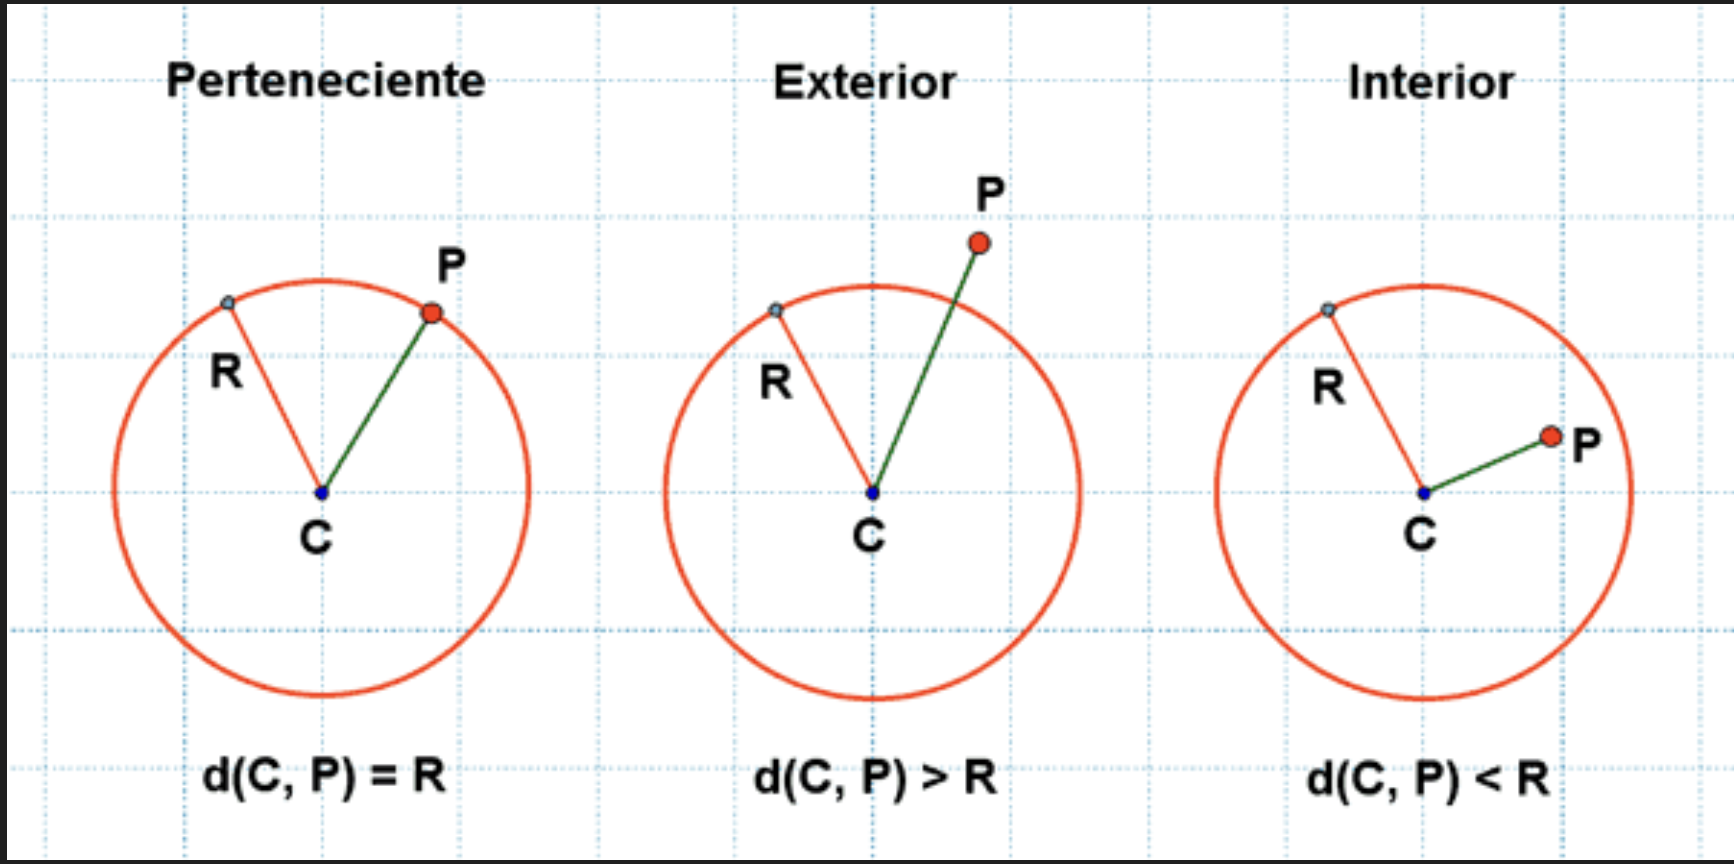
\includegraphics[width = 5 cm]{./latex-imágenes/circunferenciaE32.png}
    \caption{Ejemplo de comparación de la distancia y el radio.}
    \label{fig:uno}
\end{figure}


\subsection{\textbf{Diseño de la solución:}}

\begin{enumerate}
\item Solicitar al usuario que ingrese las coordenadas del punto $C$ y el punto $T$, es decir $(x_{1}, y_{1})$ y $(x_{2}, y_{2})$ y el radio $r$.
\item Calcular la distancia entre el centro y el punto.
\item Verificar si el punto está dentro del área de la circunferencia
\item Al final mostrar el resultado al usuario \\
\end{enumerate}

\begin{figure}[h!]
    \centering
    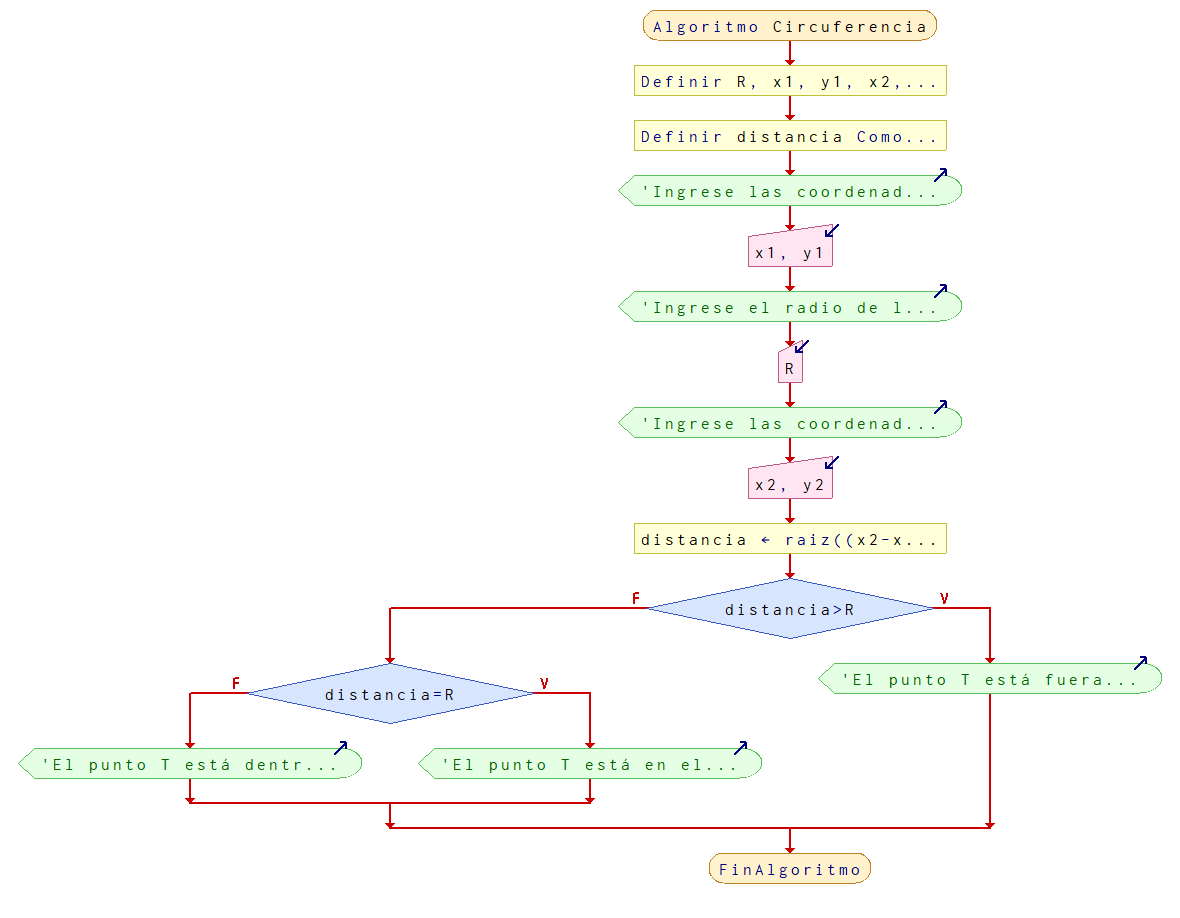
\includegraphics[width = 8 cm]{./latex-imágenes/DiagramaE3.png}
    \caption{Diagrama de flujo del problema 3}
    \label{fig:DiagrmadeFlujo}
\end{figure}


\subsection{\textbf{Desarrollo de la solución:}}

Se importa la clase Scanner para que se pueda leer las entradas del usuario
\begin{javaCode}
import java.util.Scanner;
\end{javaCode}

Posteriormente se define la clase llamada "CircufrenciaIntegrador" que contendrá el programa.
\begin{javaCode}
    public class CircuferenciaIntegrador {
    public static void main(String[] args) {} 
\end{javaCode}\\

Igualmente se crea una instancia de Scanner para leer la entrada del usuario
\begin{javaCode}
Scanner datC = new Scanner(System.in);
\end{javaCode}

Se solicita al usuario que ingrese las coordenadas del punto C en el formato \textbf{"x1, y1"}, las cuales se almacenan en un arreglo de cadenas llamado \textbf{"puntoC"}
\begin{javaCode}
System.out.print("""
                Ingrese las coordenadas del punto C 
                seperadas por una coma (x1, y1):
                         """);
    String[] puntoC = (datC.nextLine()).split(",");
\end{javaCode}

Igualmente se solicita al usuario que ingrese el $radio$ de la circunferencia, se almacena en una variable $r$ de tipo float
\begin{javaCode}
System.out.print("Ingrese el radio de la circunferencia: ");
    float r = datC.nextFloat();
    datC.nextLine();  
\end{javaCode}

Seguidamente se solicita al usuario que ingrese las coordenadas del punto T que es el punto de , en el formato \textbf{"x2, y2"} que se almacenan en un arreglo de cadenas llamado \textbf{"puntoT"}
\begin{javaCode}
//Obtener las coordenadas del punto a verificar
System.out.print("""
                Ingrese las coordenadas del punto T
                seperadas por una coma (x2, y2): 
                         """);
String[] puntoT = (datC.nextLine()).split(",");
\end{javaCode}

Se Cierra el objeto Scanner para liberar los recursos.
\begin{javaCode}
                  datC.close(); 
\end{javaCode}
Se convierte las coordenadas del punto C y del punto T de cadenas a enteros (x1, y1, x2, y2).
En Java, convertir datos en cadenas a enteros es útil cuando necesitas manipular o realizar operaciones matemáticas con números enteros que se encuentran representados como \textit{cadenas de caracteres}.
\begin{javaCode}
int x1 = Integer.parseInt(puntoC[0].trim());
int y1 = Integer.parseInt(puntoC[1].trim());
        
int x2 = Integer.parseInt(puntoT[0].trim());
int y2 = Integer.parseInt(puntoT[1].trim());
\end{javaCode}

En esta parte del desarrollo se calcula la distancia entre el centro (punto C) y el punto T utilizando la fórmula de la distancia euclidiana que significa; la distancia en línea recta entre dos puntos en un plano.
\begin{javaCode}
float distancia = (float)Math.sqrt(Math.pow(x2 - x1, 2) + Math.pow(y2 - y1, 2));   
\end{javaCode}

Al final se utiliza las condiciones \textbf{if, else if y else} para evaluar la relación entre la distancia y el radio de la circunferencia, con esto se verifica si el punto T se encuentra dentro de la circunferencia, en el borde o fuera de ella y se muestra el resultado al usuario.
\begin{javaCode}
//Verificar si el punto está dentro del área de la circunferencia
     if (distancia > r) {
    System.out.println("El punto T("+x2+","+y2+") esta fuera de la circunferencia");
    }else if (distancia == r) {
     System.out.println("El punto T("+x2+","+y2+") esta en el borde de la circunferencia");
    }else if (distancia < r){
     System.out.println("El punto T("+x2+","+y2+") esta dentro de la circunferencia"); }
\end{javaCode}

\subsection{\textbf{Depuración y pruebas:}}

\begin{table}[h!]
     \centering
     \caption{Tabla de Corridas del problema 3}\\

     \begin{tabular}{|c|c|c|c|c|c|}
     \hline
    Corrida & C$(x_{1}, y_{1})$& T$(x_{2}, y_{2})$  &  R $r$ & Resultado\\
    \hline
    1  &  $(3,4)$ & $(9,2)$ & 10 & $T$ esta adentro \\
    \hline
    2  &  $(5,2)$ & $(8,1)$ & 12 & $T$ esta adentro \\
    \hline
    3  &  $(34,23)$ & $(-90,35)$ & 67 & $T$ esta afuera \\
    \hline
    4  &  $(-27,3)$ & $(34,-5)$ & 30 & $T$ esta afuera \\
    \hline
    5 &  $(2,8)$ & $(4,9)$ & 17 & $T$ esta adentro \\
    \hline
     \end{tabular}
     \label{tab:my_label}
 \end{table}

\clearpage

\section{Resolución Problema 4}
\subsection{Problema:}
Dado un numero decimal entero positivo o negativo regresar su equivalente en binario.


\subsection{\textbf{Descripción del problema:}}
Dado un numero decimal entero positivo o negativo regresar su equivalente en binario.

\subsection{\textbf{Definición de solución:}}
El informe analiza el proceso de conversión de un número decimal entero positivo o negativo a su representación binaria. Se resalta la relevancia de comprender, en el ámbito de las matemáticas discretas, cómo un número experimenta este cambio de representación.
\newline


\item[{\ieeeguilsinglright}] {\it A. DECIMALES POSITIVOS }
   
La conversión de números decimales positivos a binarios, esta basada en divisiones sucesivas por 2. 
\newline

\begin{figure}
\centerline{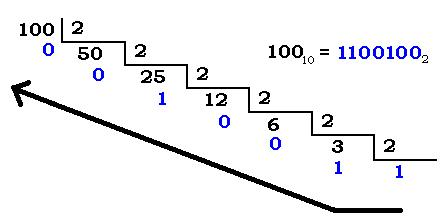
\includegraphics[width=18.5pc]{./latex-imagenes/conversion.jpg}}
\caption{Proceso de conversión de 100 utilizando la técnica de sucesivas divisiones por dos}
\vspace*{-5pt}
\label{fig:dos}
\end{figure}


\item[{\ieeeguilsinglright}] {\it B. DECIMALES NEGATIVOS }

Por n el caso de números negativos, el proceso se complica y se introduce el concepto de complemento 1 y 2.

\begin{itemize}
    \item Complemento a 1:
\end{itemize}
En el contexto del "complemento a 1" de un número binario, nos referimos a la secuencia de bits que se obtiene al invertir (cambiar de 0 a 1 y de 1 a 0) todos los bits del número original. 
\newline

Por ejemplo, si tenemos el número binario 01010101, al aplicar el complemento a 1 obtendríamos 10101010, ya que hemos invertido cada bit. El complemento a 1 se utiliza principalmente para representar la magnitud negativa de un número binario y es una parte fundamental en el cálculo del complemento a 2."
\newline

\begin{itemize}
    \item Complemento a 2:
\end{itemize}
El proceso de obtener el complemento a 2 de un número binario es un paso esencial en la representación de números negativos en sistemas binarios. Este método se basa en la utilización del complemento a 1 y la adición de 1 al resultado
\newline

\begin{figure}
\centerline{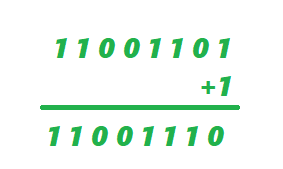
\includegraphics[width=18.5pc]{./latex-imagenes/complementoADos}}
\caption{Proceso de conversión de 100 utilizando la técnica de sucesivas divisiones por dos}
\vspace*{-5pt}
\label{fig:dos}
\end{figure}

\subsection{\textbf{Diseño de la solución:}}
\begin{itemize}
    \item Utiliza la clase Scanner para solicitar al usuario que ingrese un número decimal entero positivo o negativo en el rango de 64 bits, específicamente entre -1024 y 1024.
    \item Lee la entrada del usuario y almacena el valor en la variable numeroD.
    
    \item Convierte la cadena numeroD a un número de tipo long llamado numeroDecimal.
    \item Verifica si numeroDecimal está en el rango permitido. Si es positivo, realiza la conversión a binario. Si es negativo, calcula los complementos a uno y a dos.
    \item Si el número está fuera del rango, lanza unmensaje.
    
    \item Convierte el valor absoluto de numero a su representación binaria.
    \item Utiliza un bucle para realizar sucesivas divisiones por 2, registrando los residuos como bits en la representación binaria.
    
    \item Para complemento a Uno, utiliza la representación binaria obtenida anteriormente.
    
    \item Determina la longitud de bits necesarios para representar el número según su rango.
    
    \item Añade ceros a la izquierda para alcanzar la longitud necesaria.
    Invierte cada bit para obtener el complemento a uno.
    
    \item Para el complemento a dos utiliza la representación del complemento a uno.
    
    \item Agrega 1 al resultado para obtener la representación del complemento a dos.
    
    \item Utiliza la clase BigInteger para manejar números grandes, ya que la representación de 65 bits podría exceder la capacidad de un tipo de datos primitivo.
    
    \item Imprime el resultado de la conversión a binario o los complementos a uno y a dos, según sea el caso.
    \end{itemize}

    \begin{figure}
        \centerline{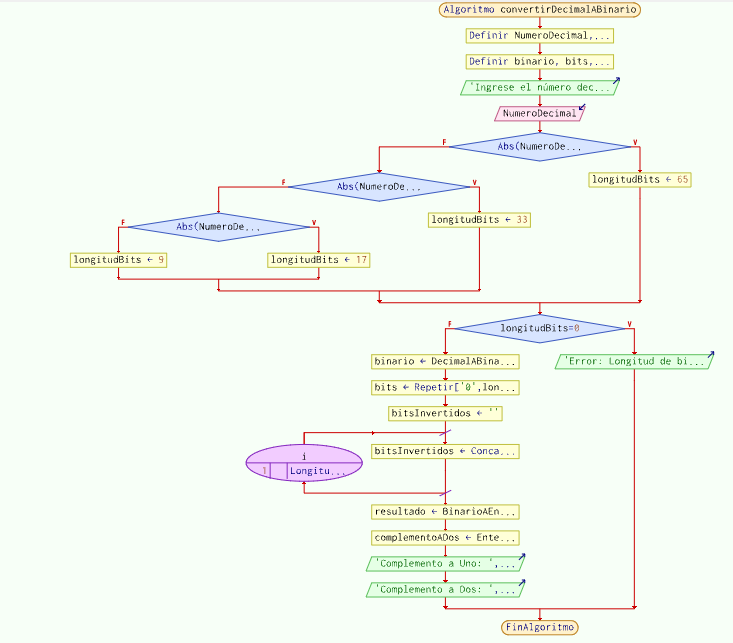
\includegraphics[width=18.5pc]{./latex-imagenes/diagramaDecimalABinarioNegativo}}
        \caption{Diagrama de flujo en caso de ser números Positivos}
        \vspace*{-5pt}
        \label{fig:dos}
        \end{figure}

        \begin{figure}
            \centerline{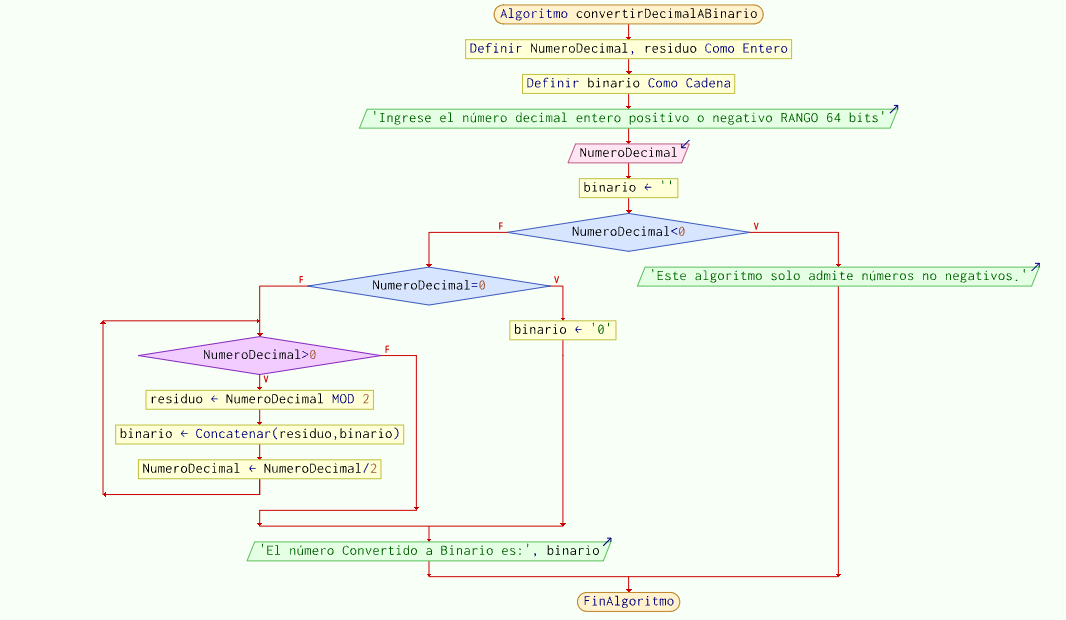
\includegraphics[width=18.5pc]{./latex-imagenes/diagramaDecimalABinarioPositivo}}
            \caption{Diagrama de Flujo en  caso de ser números negtivos }
            \vspace*{-5pt}
            \label{fig:dos}
            \end{figure}
            
            


\subsection{\textbf{Desarrollo de la solución:}}

El algoritmo de solución para la conversión 
Comienza importando librerías específicamente "Scanner" para capturar todo lo que ingrese el usuario y "BigInteger".

\begin{javaCode}
import java.math.BigInteger;
import java.util.Scanner;
\end{javaCode}

Se validan los datos, usuario tiene condiciones hacerca del numero a convertir, el numero debe ser solo entero ya sea positivo o negativo entre el rango de 64 bits, dependiendo su valor va a imprimirlo de acuerdo al numero ingresado.
Posteriormente se agrega en el método principal, la instrucción para imprimir el resultado de la conversión, en caso de ser negativo se imprimen dos casos de complemento 1 y complemento 2.

\begin{javaCode}
   public static void main(String[] args) {
        Scanner decimal = new Scanner(System.in);

        
        // Solicitud del número decimal
        System.out.println("Ingrese el número decimal entero positivo o negativo RANGO 64 bits [-1024, 1024]: ");
        String numeroD = decimal.nextLine();

        // Convierte la variable a un número de tipo long 
        numeroDecimal = Long.parseLong(numeroD);

        // Valida el rango solicitado
        if (numeroDecimal >= -1024 && numeroDecimal <= 1024) {
            if (numeroDecimal >= 0) {
                // Impresión del número convertido en caso de ser positivo 
                System.out.println("El número convertido a binario es: " + decimalABinario());
            } else {
                //Impresión del número en caso de ser negativo 
                System.out.println("Complemento a 1: " + complementoAUno());
                System.out.println("Complemento a 2: " + complementoADos());
            }
    
}
\end{javaCode}

En caso contrario que el usuario haya tecleado un numero diferente al solicitado , donde si se encuentra fuera del rango o sea otro tipo de valor va a arrojar un mensaje de "Error". 
Y cierra el escaneo para seguridad.

\begin{javaCode}
    //Excepción en caso de no encontrase en el rango solicitado
    } else {
         System.out.println("Error: Formato no válido" );
    }
// Cerrar el scaneo 
decimal.close(); 
\end{javaCode}

En el método decimalABinario se crea una variable llamada "binario" es una cadena,  toma el valor decimal y lo convierte en el valor absoluto, automáticamente si el numero ingresado es 0 lo retornara de igual forma 

\begin{javaCode}
    public static String decimalABinario() {
        String binario = "";
        // Convetir decimal a valor absoluto 
        long numero = Math.abs(numeroDecimal);

        if (numero == 0) {
            return "0";
        }
\end{javaCode}


Después se crea un bucle para los números diferentes de 0, como el número ya se convirtió e absoluto este ahora podrá tomar tanto números negativos como positivos para convertirlos, el bucle didive entre 2 y su residuo lo concatena de derecha a izquierda, retornando su valor a 0.

\begin{javaCode}
     // Bucle para convertir a número decimal
        while (numero != 0) {
            long residuo = numero % 2;
            binario = residuo + binario;
            numero = numero / 2;
        }
        return binario;
    }
\end{javaCode}
De acuerdo al número ingresado a partir de if se comparara su rango, si es de 128 a -128 corresponde a 8 bits y asi sucesivamente  pero como es necesario realizar una suma para el complemento 2, este en lugar de tener 8 en su lugar camiara a 9.

\begin{javaCode}

    public static String complementoAUno() {
        // Obtener la representación binaria del número absoluto
        String binario = decimalABinario();

        // Determinar la longitud de bits necesarios
        int longitudBits;
        if (numeroDecimal >= -128 && numeroDecimal <= 128) {
            longitudBits = 9;
        } else if ((numeroDecimal >= 129 && numeroDecimal <= 256) || (numeroDecimal >= -256 && numeroDecimal <= -129)) {
            longitudBits = 17;
        } else if ((numeroDecimal >= 257 && numeroDecimal <= 512) || (numeroDecimal >= -512 && numeroDecimal <= -257)) {
            longitudBits = 33;
        } else if ((numeroDecimal >= 513 && numeroDecimal <= 1024) || (numeroDecimal >= -1024 && numeroDecimal <= -513)) {
            longitudBits = 65;
        } else {
            return "Error";
        }
\end{javaCode}

Se ajusta la longitud de la cadena binaria añadiendo ceros a la izquierda según sea necesario. Luego, se itera sobre cada bit en la cadena, invirtiéndolos y construyendo así la representación del complemento. La utilización de StringBuilder mejora la eficiencia en la manipulación de cadenas dentro del bucle. Finalmente, se retorna la representación del complemento a uno como una cadena de texto.

\begin{javaCode}
   // Añadir ceros a la izquierda según la longitud necesaria
        String bits = "0".repeat(Math.max(0, longitudBits - binario.length())) + binario;

        // Añadir ceros a la izquierda según la longitud necesaria
        String bits = "0".repeat(Math.max(0, longitudBits - binario.length())) + binario;

        // Invertir cada bit guardandolo en complemento 
         StringBuilder complemento = new StringBuilder();
        for (int i = 0; i < bits.length(); i++) {
            char bit = bits.charAt(i);
            complemento.append((bit == '0') ? '1' : '0');
        }

        return complemento.toString();
    }
\end{javaCode}


\begin{javaCode}
       public static String complementoADos() {
        // Obtener la representación del complemento a uno
        String binario = complementoAUno();

        // Agregar 1 al resultado para obtener la representación de complemento a 2
        //Declarar el resultado en BigInterger para numeros de 65 bits
        BigInteger resultado = new BigInteger(binario, 2).add(BigInteger.ONE);
        return resultado.toString(2);
    }
\end{javaCode}


\subsection{\textbf{Depuración y pruebas:}}


\begin{center}
    \textbf{Tabla de Números Positivos}
    
    \begin{tabular}{|c|c|c|c|}
    \hline
    \textbf{Entrada Decimal} & \textbf{Binario Resultante} \\
    \hline
    7 & 111 \\
    \hline
    10 & 1010 \\
    \hline
    0  & 0  \\
    \hline
    \end{tabular}
\end{center}

\begin{center}
    \textbf{Tabla de Números Negativos}
    
    \begin{tabular}{|c|c|c|c|}
    \hline
    \textbf{Entrada Decimal} & \textbf{Complemento a Uno} & \textbf{Complemento a Dos} \\
    \hline
    -4 & 111111011 & 111111100 \\
    \hline
    -124 & 110000011 & 110000100\\
    \hline
    \end{tabular}
\end{center}

\clearpage

\section{Resolución Problema 5}
\subsection{Problema:}
Dado un numero binario de $n$ bits regresar su equivalente en decimal.

\subsection{\textbf{Descripción del problema:}}

El reporte analiza el concepto de ingresar un número de tipo binario con $n$ bits, para posteriormente regresar su equivalente en decimal.

\begin{figure}[h!]
    \centering
    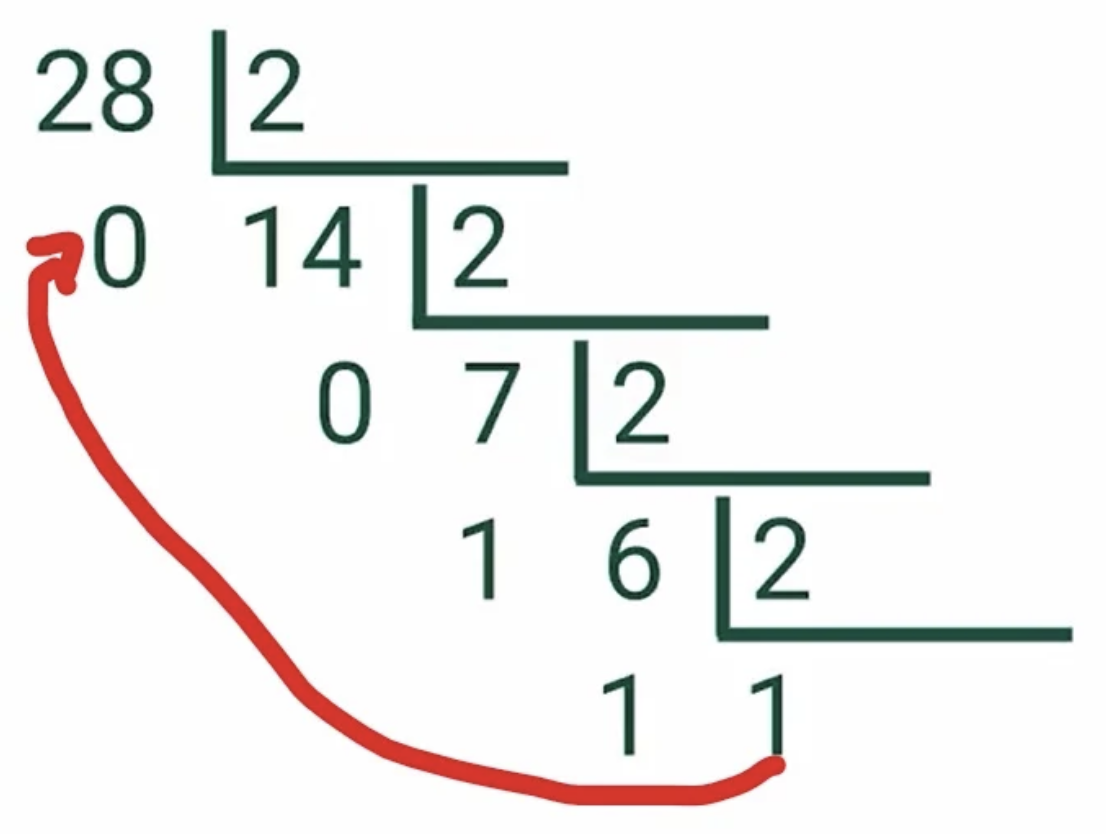
\includegraphics[width = 6 cm]{./latex-imágenes/conversionbin5.png}
    \caption{Conversión de binario a su equivalente decimal}
    \label{fig:GraficaEcuacionRecta}
\end{figure}

\subsection{\textbf{Definición de solución:}}

Los números binarios se conforman con los símbolos 0 y 1, que se combinan para representar cualquier número. 
Para representar números superiores a 1 dígito, se aplica un método semejante al de formación de números decimales, combinando ordenadamente los símbolos. Se repiten las combinaciones de dígitos anteriores y se le añade un dígito para continuar la numeración

\begin{table}[h]
     \centering
     \caption{Valores binarios}
     
     \begin{tabular}{|c|c|}
     \hline
        Corrida & Binario \\
        \hline
        0  & 0 \\
        \hline
        1  & 1 \\
        \hline
        2  & 10 \\
        \hline
        3  & 11 \\
        \hline
        4  & 100 \\
        \hline
        5  & 101 \\
        \hline
        6  & 110 \\
        \hline
        7  & 111 \\
        \hline
        8  & 1000 \\
        \hline
        9  & 1001 \\
        \hline
        10  & 1010 \\
        \hline
        11  & 1011 \\
        \hline
        12  & 1100 \\
        \hline
     \end{tabular}
     \label{tab:my_label}
 \end{table}

En el sistema binario se utiliza la ponderación por posición de dígito en la misma forma que en la numeración decimal, por ejemplo:

\begin{table}[h!]
     \centering
     \caption{Ponderaciones}
     
     \begin{tabular}{|c|c|c|c|c|}
     \hline
        Posición & 3 & 2 & 1 & 0 \\
        \hline
        ponderacion  & 2^{3} & 2^{2} & 2^{1} & 2^{0} \\
        \hline
        Peso en decimal  & 8 & 4 & 2 & 1 \\
        \hline
        Número en binario  & 0 & 1 & 0 & 1 \\
        \hline
     \end{tabular}
     \label{tab:my_label}
 \end{table}

El resultado da la operación se obtiene de hacer la operación “res=0*8+1*4+0*2+1*1”

\subsection{\textbf{Diseño de la solución:}}

\begin{figure}[h!]
    \centering
    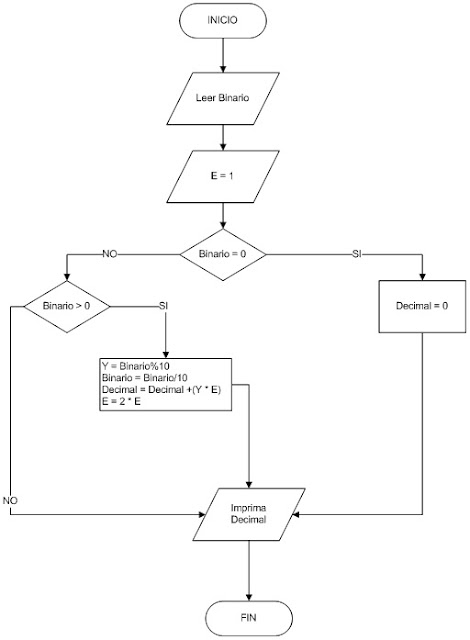
\includegraphics[width = 6 cm]{./latex-imágenes/dflujo5.jpg}
    \caption{Diagrama de flujo de el algoritmo de solución}
    \label{}
\end{figure}

\begin{enumerate}
    \item Solicitar al usuario que ingrese el número binario de n bits.
    \item Validar que el número binario ingresado sea válido, es decir, que esté compuesto únicamente de 0's y 1's y tenga una longitud de n bits.
    \item Calcular el número decimal equivalente utilizando el método binAdecimal.
    \item Mostrar el resultado al usuario.
\end{enumerate}

\subsection{\textbf{Desarrollo de la solución:}}

El algoritmo de solución del problema comienza solicitando al usuario teclee el número binario a convertir, para posteriormente almacenarlo en la variable $nbinario$.
\begin{javaCode}

Scanner in = new Scanner(System.in);
        
    System.out.println("ALGORITMO PARA CONVERTIR UN NÚMERO BINARIO A DECIMAL");
    System.out.println("------");
    System.out.println("Ingresa el número binario correspondiente: ");
    String nbinario = in.nextLine();
    in.close();
        
\end{javaCode}

Se inicializa un $if$, esto con la finalidad de que si se llega a ingresar el signo "-", la conversión lo elimine.

\begin{javaCode}

if (nbinario.contains("-")) {
    nbinario = nbinario.replace("-", "");
    }

\end{javaCode}

Posteriormente, se vuelve a inicializar un $if$, este para realizar la operación de conversión únicamente si el dato de entrada contiene 0 y 1, de lo contrario, cancelar la conversión arrojando un mensaje de error.

\begin{javaCode}

if (nbinario.matches("[01]+")) {
    int num = binAdecimal(nbinario);
    System.out.println("Número decimal: " + num);
    }else{
        System.out.println("Carácter de tipo inválido");
    }
\end{javaCode}

Si la condición anterior se cumple, se manda a llamar al método $binAdecimal$, que es el que contiene todo el proceso de conversión.
\begin{javaCode}

public static int binAdecimal(String binario) {
    int n = binario.length();
    int decimal = 0;
       
    for (int i = 0; i < n; i++) {
        int bit = 
        Character.getNumericValue(binario.charAt(i));
    decimal += bit * Math.pow(2, n - 1 - i);
    }

    return decimal;
}
    
\end{javaCode}

\subsection{\textbf{Depuración y pruebas:}}

\begin{table}[h!]
     \centering
     \caption{Tabla de Corridas}\\
     
     \begin{tabular}{|c|c|c|}
     \hline
        Corrida & Binario & Decimal\\
        \hline
        1  & 010111 & 23\\
        \hline
        2  & 011011 & 27\\
        \hline
        3  & 101010 & 42\\
        \hline
        4  & 010101 & 21\\
        \hline
        5  & 111011 & 59\\
        \hline
     \end{tabular}
     \label{tab:my_label}
 \end{table}
\vspace*{-8pt}
\clearpage

\section{Resolución Problema 6}

\subsection{\textbf{Descripción del problema:}}

\subsection{\textbf{Definición de solución:}}

\subsection{\textbf{Diseño de la solución:}}

\subsection{\textbf{Desarrollo de la solución:}}

\subsection{\textbf{Depuración y pruebas:}}
\clearpage


\section{CONCLUSION}
El manuscrito debe incluir direcciones futuras de la investigación. Se recomienda encarecidamente a los autores que no hagan referencia a varias figuras o tablas en la conclusión; estos deben mencionarse en el cuerpo del artículo.
\vspace*{-8pt}


\section{AGRADECIMIENTOS}
Esta sección es opcional. Si los autores creen necesario agradecer a alguien por haber aportado al desarrollo de su proyecto integrador de alguna u otra forma, esta sección esta destinada para esto.


\def\refname{REFERENCES}

\begin{thebibliography}{1}

\bibitem{AA1}
G. M. Amdahl, G. A. Blaauw, and F. P. Brooks, ``Architecture of the IBM System/360,'' {\it IBM J. Res. Dev}., vol. 8, no. 2, pp. 87--101, 1964. (Journal)

\bibitem{BB1}  
Cunoticias. (s. f.). Complemento a 1 (uno) con ejemplos. https://www.cunoticias.com/internet/complemento-a-1-uno-con-ejemplos.php

\bibitem{CC1}
Johnsonbaugh, R. (s. f.). MATEMÁTICAS DISCRETAS. Pearson Educación.

\bibitem{DD1}
Fernández, M. Y. A., Hernández, Y. J. S., & Montaña, M. M. (s. f.). Matemáticas Discretas:: Con un enfoque desde la ingeniería y ciencias sociales - Conceptos básicos. Editorial de la Universidad Pedagógica y Tecnológica de Colombia - UPTC.

\bibitem{BB1}
Sección 5: Soto, J. A. - GEEKNETIC. (Cómo convertir binario en decimal paso a paso). [Online]. Available: {https://www.geeknetic.es/Guia/2667/Como-convertir-binario-en-decimal-paso-a-paso.html} (URL)

\bibitem{CC1}
Sección 5: Escobar, B., & Perfil, V. T. mi. - Blogspot.com.. (Algoritmo para pasar de Binario a Decimal.). [Online]. Available: {http://mensajeseintereses.blogspot.com/2011/10/2-algoritmo-para-pasar-de-binario.html} (URL)

\end{thebibliography}\vspace*{-8pt}


\begin{IEEEbiography}{Cuadros Romero Francisco Javier}{\,}Todas las biografías se limitan a un párrafo y deben ser muy sintéticas. Se puede agregar la carrera en la cual el estudiante esta enrolado. Se pueden mencionar los 3 intereses principales del estudiante. Asi como su aspiración en el corto y mediano plazo. Al final de la biografia de cada estudiante se debe agregar el enlace a su pagina personal en Github: 
%\vadjust{\vfill\pagebreak}
\end{IEEEbiography}

\begin{IEEEbiography}{Karen Perez Ortiz}{\,}Originaria de Mixquiahuala de Juarez, es una estudiante de Ingeniería en Tecnologías de la Información y Comunicaciones cuyo interés por la tecnología floreció durante la secundaria, gracias a una reveladora convención tecnológica. Fascinada por la versatilidad creativa que una computadora puede ofrecer, se sumerge en la exploración de diversas ramas tecnológicas. Más allá de su dedicación académica, disfruta de series animadas, la astronomía y seguir a streamers. Con metas ambiciosas, no solo aspira a concluir la universidad, sino también a dejar un legado significativo en el campo. Su enfoque se centra en el desarrollo web con énfasis en Experiencia de Usuario (UX), y su entusiasmo por la Inteligencia Artificial y el Aprendizaje Automático la impulsa a profundizar constantemente en estos campos, motivada por la perspectiva de contribuir al avance tecnológico. https://karenperezor.github.io/.
\end{IEEEbiography}
\begin{IEEEbiography}{Neri Pérez Giovany Humberto}{\,}es un estudiante de la ingeniería en Tecnologías de la Información y Comunicaciones con una pasión desbordante por los videojuegos, el anime y los ``corridos tumbados''. Nacido y criado en  Tetepango, desde temprana edad mostró un gran interés por la tecnología y los avances en el campo de la informática. Aunque sus intereses pueden parecer diversos, Giovany encuentra inspiración en la creatividad y la narrativa tanto de los videojuegos como del anime. Estos medios le han enseñado la importancia de la perseverancia, la resolución de problemas y el trabajo en equipo. El objetivo principal de Giovany es completar sus estudios universitarios en ITICs, con especialización en ciberseguridad. Sueña con trabajar en el campo de la ciberseguridad, protegiendo sistemas e información vital de ataques cibernéticos y contribuyendo así a la seguridad digital de las organizaciones.
\end{IEEEbiography}

\end{document}

